\section{Experiment Setup}
This sections explains in detail the data collection stage and system setup.

\subsection{Seed Domain Collection}
During the data collection stage, we focused on collecting domains that serve advertisements via push notifications. Therefore, to start with, we manually browsed Google for a list of ad networks that are known to serve ads via push notifications. Then, we manually signed up as a publisher with each of these ad networks to obtain the script code that needs to be added to a website to enable the ad network's service. Later, we formed a list of certain keywords from each script that uniquely points to their associated ad network. We then use the keywords to obtain a list of domains that possibly use the ad network that the script belongs to. We searched for domains that contains keywords pointing to an ad network by using the service of source code engine, \texttt{publicwww.com} \ref{publicwww}. At this point, we had a list of 1,75,939 domains to start our analysis and the distribution of domains along with the seed keyword used to obtain them is shown in table \ref{seedDomains}.


\begin{table}[htbp]
\caption{Seed Domain Details }
\begin{center}
\label{seedDomains}
\begin{tabular}{c|c|c|c}
\toprule
\hline
\multirow{4}*{\textbf{Ad Network/Seed Keyword}} & \multicolumn{3}{c}{\textbf{Domains Count}} \\ 
\cline{2-4}
~ & \textbf{HTTPS} & \textbf{HTTP} & \textbf{\makecell{HTTPS \\Notification \\Permission}}\\
\hline
 \hline
 cloudfrontnet & 49769 & 50148 & 1394
 \\
 \hline
 cdnpushcrewcomjs & 15177 & 5143 & 478
 \\
 \hline
 cdnonesignalcomsdk & 11317 & 7241 & 3149
 \\ 
 \hline
 NotificationrequestPermission & 3965 & 6417 & 562
 \\ 
 \hline
 pushmanagersubscribe & 2667 & 800 & 173
 \\ 
 \hline
 popadsnet & 1581 & 8154 & 80
 \\ 
 \hline
 apipushengagecom & 796 & 896 & 238
 \\ 
 \hline
 cdnizootocomscripts & 676 & 625 & 301
 \\ 
 \hline
 pubmaticcomAdServer & 647 & 230 & 8
 \\ 
 \hline
 adnetworkpropellerads & 335 & 740 & 10
 \\ 
 \hline
 addEventListenerpush & 250 & 43 & 9
 \\ 
 \hline
 criteocomdeliveryajsphp & 154 & 1540 & 5
 \\ 
  \hline
 terraclickscom & 86 & 662 & 0
 \\ 
  \hline
 adsblockkpushcom & 55 & 4235 & 21
 \\ 
  \hline
 airpush & 52 & 169 & 0
 \\ 
  \hline
 puservingcom & 29 & 628 & 2
 \\ 
   \hline
 hilltopadsnet & 21 & 160 & 3
 \\  
   \hline
 adsad4gamecomwww & 14 & 179 & 0
 \\   \hline
 richpush & 12 & 10 & 0
 \\   \hline
 adcashcomscriptjava & 10 & 258 & 0
 \\   \hline
 jspushmonetizationcom & 9 & 14 & 5
 \\ 
 \hline
 \bottomrule
    \end{tabular}
\label{tab1}
\end{center}
\end{table}

\subsection{Filtering Seed Domains}
As a first stage of processing, we filtered the list of seed domains collected to retain only those that request for notification permission. To achieve this, we visited each of the seed domains using our framework \sysname. The log generated by the Chromium component records any request for notification permission. Thus, we parse the logs to check if a request to notification permission was made. Only those domains that request to send notifications to users are retained for the next stage of processing. The number of domains that requests notification permission is shown in table \ref{seedDomains}

\subsection{Monitoring Notifications : Desktop Environment}
In desktop environment of \sysname, we use docker containers  to monitor notifications. For each domain that has to be monitored, a docker container is created to provide a virtual environment. As we create separate containers for each domain, it prevents ad networks from fingerprinting the user using any third party cookies and other user based information. Further, it also allows us to visit multiple domains in parallel increasing the rate of our experiment. Since we already filtered the domains that request for notification, we proceed with the monitoring phase as follows

\begin{itemize}
    \item First, we create a new docker container for each domain that needs to be monitored. This docker container already has the modified Chromium installed in it. 
    \item We execute a nodejs script that uses puppeteer tool to automatically control the Chromium browser in each container. This script starts Chromium browser and opens the website URL that is passed to it on a new tab. By default, service worker  gets registered and Chromium grants permission for notification to the website. In order to allow time for the website to load, register it's service worker and request permission, the web page is kept open for until 5 minutes. 
    \item At this point, after the service worker is registers, the docker container is kept alive for 15 minutes. In a desktop environment, for Chromium browser to receive push messages, the browser process needs to be running. Hence, even though we close the web page after 5 minutes, we keep the browser process running. It is essential to close the web page after 5 minutes because, it is possible that the website won't send any notification as long as the web page is open.
    \item After 15 minutes of monitoring the docker container, we stop the container and proceed with monitoring next URLs. Stopping the container frees both CPU and memory used by the container and its process. However, the container could be started at any point of time to resume the operation.
    \item After a certain period of time, we resume the stopped container and execute the nodejs script to open the browser process. Since this browser process uses the same user profile, the permission provided previously applies to this session. However, service workers are designed to become inactive after a certain period of time. Service workers are activated whenever a push message is sent to them. Therefore, whenever a push message is sent by the messaging server, the service worker is activated and it continues with the process of displaying notifications.
    \item Whenever we resume a container and start the browser process, it tends to display all the queued notifications 3 at a time. But all these queued notifications would be added at the same time as soon as the browser is active. Since, our system is designed to emulate a click 15 seconds after it gets added, some notifications might be clicked even before they get displayed. To resolve this issue, we modified Chromium code to induce a delay of 10seconds whenever it adds a notification using the \texttt{MessageCenterNotificationManager.Add} module. This ensures that all queued notifications are displayed before a click is emulated.
    \item A resumed container is kept open for 15 minutes and stopped to be resumed at a later point of time. This helps to mimic an user's behavior of closing the browser or staying logged off for specific duration in a day. Also, this allow us to efficiently utilize the system resources to monitor next set of URLs. 
    \item The executed nodejs script and the modified Chromium records every interaction as mentioned in system overview. This includes capturing a screenshot of every web page that opens and the notifications that get displayed. The logs collected through the script and Chromium tool provide us a fine-grained detail of the execution of web page and the service worker involved. 
\end{itemize}

%%%%%%%%%%%%%%%%%%%%%%%%%%%%%%%%%%%%%%%%%%%%%%%%%%%%%%%%%%%%%%%%%%%
\subsection{Monitoring Notifications: Mobile Environment} \label{monitoring}
In mobile environment of \sysname, We had to take into consideration the device's physical and technical limitations. \st{In order to collect website notifications from mobile environment, there are two ways that we took into consideration.}\samuel{The reasons we are collecting website notifications from a real mobile device are because} 1) To use the feature in desktop Chromium that could change the view to a mobile view to collect ads in mobile environment. \samuel{Website can easily detect whether the environment is mobile or not(citations). And based on our observation, advertisement network would send out mobile-specific advertisements to attract uses' attention. } 2) Since most of the websites now use advanced tracking methods to determine if a mobile user is legit by monitoring various sensors such as acceleration, orientation, location etc., \samuel{In order to lower the risk of losing notifications, }we chose \st{the later option} to run experiments on a real android device. Also, in android devices sometimes, they look for google play services which could not be simulated using a \warn{Chromium mobile view}(\samuel{This term is not easy to understand I think}). 

\samuel{However in mobile environment of \sysname, We had to take into consideration the device's physical and technical limitations. 
 Certain physical features of a mobile device such as memory and CPU processing restrict the number of URLs that we could monitor over a period of time compared to desktop setup. In order to collect notification in an efficient way, we open multiple URLs in one chromium application. Even though the logs are mixed in one log file, we still can separate logs from different websites later using the parser. We use a Nexus 5 running AOSP(Android Open Source Project) version 7.1.1\_r38 with Open GApps\cite{gapps} installed.} The procedure followed in collecting notifications on a mobile device are listed below.   
\begin{enumerate}
    \item First, we install modified Chromium and our app on the device using the command below. \samuel{The parameter \texttt{-g} is to grant chromium all the application level permissions it might ask for later. There are two levels of permissions in chromium. First is application level permissions, which are controlled by Android Operating System. Second is website level permissions, which are managed by chromium. The application level permissions are shared within all the websites inside chromium. However, chromium still would ask for user's consent for website level permission if the website is asking for sensitive information, like in fig. \ref{website_level_permission}. We granted the application level permissions during installing time of chromium \warn{ and granted website level permissions through modifying chromium source code}. \\
        \texttt{adb install -g MonochromePublic.apk}}
    \item Next, we create a custom browser setting profile and push it into the device using ADB. In the setting profile, we turn off third party cookies, safe browsing, data saver, and other options that might interfere the data collection. As we cannot sandbox each URL's visit in a mobile environment, turning off third party cookies would prevent same ad network used by different domains \st{that we visit} to fingerprint the user. Once an ad network fingerprints the mobile device as a single user, it might hinder the number of ads that are delivered to the device by the ad network. \st{Further,}Google's safe browsing might block websites that are on our list if it deems them malicious and this would limit our domain pool. On data saver mode(renamed lite mode in recent releases), some of the web traffic may go through Google servers before reaching the device. We turned off this option in case Google servers have safety mechanism to block malicious websites\samuel{, or in some cases, Google may modify/compress the website's source code in order to make it faster to load. }.
    \item \label{spawn_website} Then, we connect the device to a computer in order to control the device using ADB. We use the following ADB command on the connected computer to start Chromium and visit a domain on the device. 
        \texttt{adb shell am start -n \path{org.chromium.chrome/org.chromium.chrome.browser.ChromeTabbedActivity} -d [URL] --es \path{"com.android.browser.application_id"} "com.package.name"}
    \item At this point, logs printed to \texttt{logcat} from Chromium app are piped into our log file. At the same time, we are monitoring the CPU load using the following command.\\
        \samuel{\texttt{adb shell uptime}}
    \item After visiting a page, we waited for 5 minutes to allow for the website to load, successfully register service worker and gain permission to request notification. This time interval was determined based on our observations that is shown in Fig. \ref{sw_reg_time}. 
    \item After 5 minutes, we proceed with visiting next URL on a new page using the command in Step \ref{spawn_website}. Any service workers that were registered by previously visited sites would be running in the background.
    \item After we open all the pages, we wait for 5 days to receive notifications. 
\end{enumerate}

\begin{figure}[h]
\begin{center}
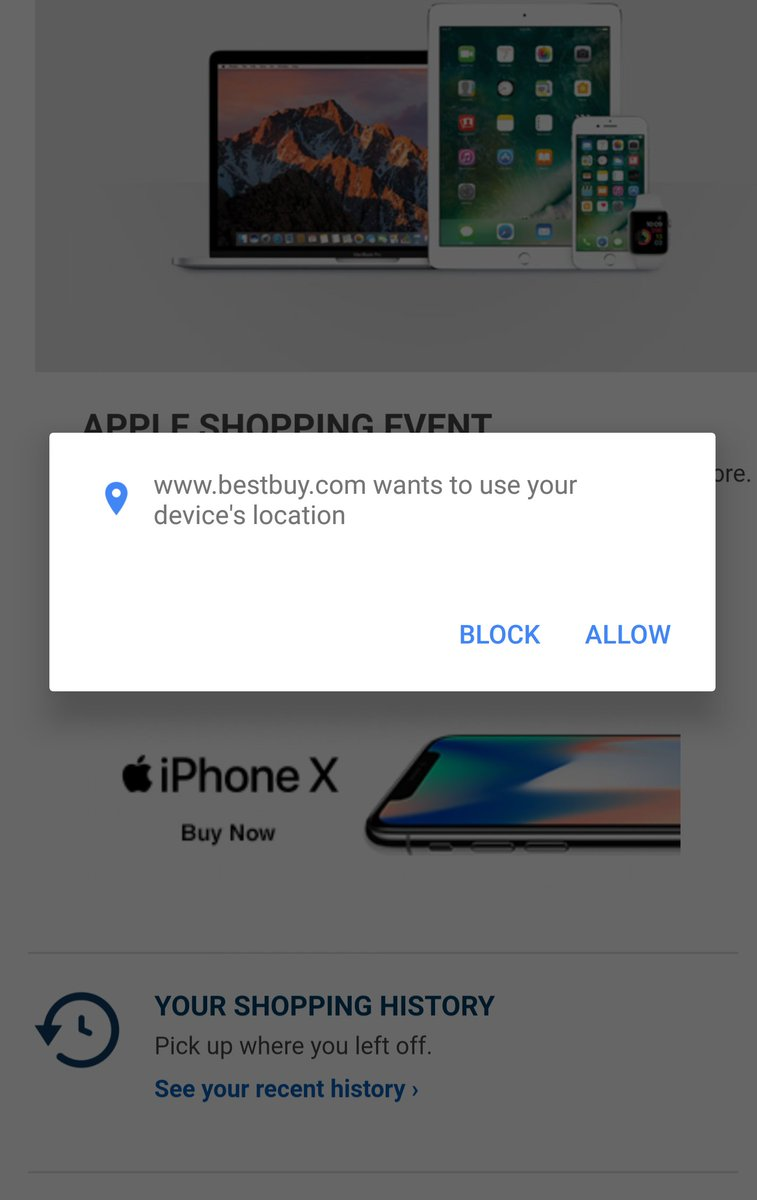
\includegraphics[scale=0.25]{figs/website_level_permission.jpg}
\caption{Example of website level permission on mobile device.}
\label{website_level_permission}
\end{center}
\end{figure}

At any point during this experiment, the mobile device can run out of battery as it is only charged through the USB connected to the computer \samuel{(approximately 0.5A/5V)} that controls the device using ADB. Under such circumstances, our experiments would be stopped abruptly. In order to overcome this problem, we monitor the device's battery level and when it is below a certain level \samuel{we pause the android device using \\\texttt{adb shell stop}\\ and resume it once the device is fully charged using \\\texttt{adb shell start}\\ The advantage of using these commands is we can still using ADB to monitor the device battery information while the essential components, including Zygote(core process of Android applications), SystemServer and SurfaceFlinger(display)\cite{android_graphics}, are stopped.} Once resumed, the processes continue with their operations as though there was no delay involved. \warn{Although the previous notifications are cleared out. But I guess we don't need to mentioned them... or do we?}

\subsection{Parsing Logs: Desktop Environment}
After we run the experiments, we obtain a chromium log file for every docker container session. This log generated by Chromium is very detailed as they contain fine-grained information about all DOM modifications, Notification related calls and events, critical JS
API calls and parameters etc. Therefore, we parse the log file to filter out any redirection, service worker registration, subscription keys,notification permission request, notification events such as show, click and close, API calls made by service worker and tab open. We record the filtered log entries and attributes related to each entry in a database. Note that the log generated from a single docker session may have information about multiple websites. For example, If we initially visit a website ABC.com and after clicking the notification received from ABC.com, we were redirected to XYZ.com and XYZ.com also has a notification service, then our log would contain the information for both ABC.com and XYZ.com. Additionally, in desktop environment, we save any resources that are requested by the service worker such as javascript files, image files etc. We parse these resource files to fetch any URLs that are found in them and also calculate the hash of files and store them in the database for further analysis.


\subsection{Parsing Logs: Mobile Environment}
\samuel{I think we can say mobile and Desktop are basically using the same parser. That's the beauty of our tools, right?}